\documentclass[varwidth=true, border=2pt]{standalone}
\usepackage{tikz}
\usetikzlibrary{calc,shadings}
\usepackage{pgfplots}

\begin{document}
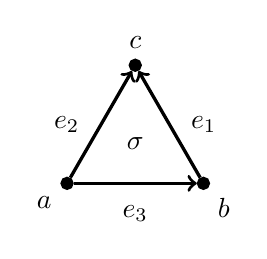
\begin{tikzpicture}
    \tikzstyle{point}=[circle,thick,draw=black,fill=black,inner sep=0pt,minimum width=4pt,minimum height=4pt]
    \node (a)[point,label={[label distance=0cm]210:$a$}] at (210:1cm) {};
    \node (b)[point,label={[label distance=0cm]-45:$b$}] at (330:1cm) {};
    \node (c)[point,label={[label distance=0cm]90:$c$}] at (90:1cm) {};

    \node (sigma) at (0,0) {$\sigma$};

    \draw[->, very thick] (a) edge node[label=below:$e_3$]  {} (b);
    \draw[->, very thick] (b) edge node[label=right:$e_1$]  {} (c);
    \draw[->, very thick] (a) edge node[label=left:$e_2$]  {} (c);
\end{tikzpicture}
\end{document}
